\documentclass[11pt]{article}
\usepackage{graphicx}
\usepackage{geometry}                		% See geometry.pdf to learn the layout options. There are lots.
                 		% ... or a4paper or a5paper or ... 
%\geometry{landscape}                		% Activate for rotated page geometry
%\usepackage[parfill]{parskip}    		% Activate to begin paragraphs with an empty line rather than an indent
			% Use pdf, png, jpg, or eps§ with pdflatex; use eps in DVI mode
								% TeX will automatically convert eps --> pdf in pdflatex		
\usepackage{amssymb}
\usepackage{float}
\usepackage{caption}
\usepackage{subcaption}
\usepackage{amsmath}
\usepackage{amssymb}


\begin{document}

\section{UI}
\begin{enumerate}
	\item[GETRNG:] Load the camera range into the UI engine from the file on the Yun sd card. (range.txt)
	\item[GETPOS:] Load the camera position into the UI engine from the file on the Yun sd card. (position.txt)
	\item[GETALGN:] View the camera alignment position stored on the Yun sd card.
	\item[SETALGN:] Write the current position as the alignment position to the Yun sd card. (alignment.txt)
	\item[Vertical:] Move all three motors.
	\item[Pitch:] Move motor A in the requested direction. Move motor B in the opposite direction.
	\item[Roll:] Move both motors A and B in the same direction/
	\item[A only:] Move only motor A.
	\item[B only:] Move only motor B.
	\item[C only:] Move only motor C.
	
	\item[Setting Range:] If for some reason the range hasn't been set correctly, do the folowing:
	\begin{enumerate} 
		\item[1.]SSH into the Yun.
		\item[2.]Use vi to manually change the position.txt file (in /mnt/sda1/) to "20000L20000L20000".
		\item[3.]Use vi to manually change the range.txt file (in /mnt/sda1/) to "20000L20000L20000".
		\item[4.]Use the webpage to move the camera all the way back to the -Z limit.
		\item[5.]Change the position.txt file to "0L0L0".
		\item[6.]Use the webpage to move the camera all the way to the +Z limit.
		\item[7.]Hit GETPOS on the webpage.
		\item[8.]Manually change the range.txt file to the current position.
	\end{enumerate}
\end{enumerate}
\begin{figure}[h]
\begin{center}
\includegraphics[width = 2in]{camerapic.png}
\end{center}
\caption{}  
\label{fd2}
\end{figure}

\section{Alignment Procedure}
\begin{enumerate}
	\item Navigate to the MotionControl webpage from the (arduino ip)/sd webpage.
	\item Navigate to the alignment mode webpage (password is cta).
	\item Use the webpage to move the camera to a position where it is aligned.
	\item Hit SETALGN to save the alignment position.
\end{enumerate}
\section{Troubleshooting}
If power is lost at any time, it might be the case that one of the following files gets deleted: position.txt, range.txt, alignment.txt\\[15pt]
Each of these files sits inside the directory /mnt/sda1\\[15pt]
If position.txt, or range.txt is missing:
\begin{enumerate}
\item[1.] Go into alignment mode if not there already and find the camera range (see "Setting Range" above).
\item[2.] Hit GETALGN to request the stored alignment position.
\item[3.] Manually move the camera to the alignment position.
\item[4.] Go back to the normal operation mode.
\end{enumerate}
If alignment.txt is missing realign the camera. Sorry :/. (This should never happen)

\section{Replacing a Yun}
\begin{enumerate}
\item[1.]Plug Yun into laptop via micro usb.
\item[2.] Look for the Yun's wifi network. If it doesn't appear, wold the wlan reset button until it blinks.
\item[3.] If the Yun's wifi network still doesn't appear try plugging the Yun ethernet into your LAN and connect to the Yun or Linino's network. Continue below as appropriate.\\
\item[\textbf{Linino} 4.] Open a browser and go to 192.168.240.1 and login to the Linino web UI. The default password is 'doghunter'.
\item[\textbf{Arduino} 4.] Open a browser and go to arduino.local and login to the Arduino web UI. The default password is 'arduino' or 'arduino1'.\\
\item[\textbf{Continue Here} 5.] Click on the advanced configuration at the top of the page.
\item[6.] Go to the network tab and click edit on the WAN panel.
\item[7.] Switch the network protocol to static ip.
\item[8.] Enter LAN ip reserved for the Yun along with the gateway ip and network mask. Hit save.
\item[9.] If required go to the wifi panel and disable the wifi.

\item[10.] If desired, set up the LAN to forward incoming requests from some port to the Yun ip.\\
\item[\textbf{Loading the sketch} 11.] If the previous Yun's sd card is still accessible just put it into the new Yun. Otherwise get a fresh sd card and download the Yun sd expander sketch (Google it).
\item[12.]If necessary find the Yun's ip address on the LAN and go that ip in your web browser. Then open up the Arduino ide and select that same ip as the port. Upload the sd expander (and or the motion control sketch) if necessary.
\end{enumerate}
\section{Tools}
\begin{enumerate}
	\item[]Bolts for ball joint mount: 5/16 inch allen
	\item[]Screw assembly bolts: 7/32 inch allen 
	\item[]Slides: 2.5 mm allen
	\item[]Screw Flange bolts: 7/16 inch wrench (2x)
	\item[]Ball joint centering screws: 3/4 inch flexible ratchet wrench with tape
	\item[]Set screws for motor pins: 1/16 inch allen
	\item[]Everything else: Phillips or flathead screwdriver
\end{enumerate}
\section{Removing the Inner Camera Structure}

Here's what I have... we need to note that a lifting crane is absolutely necessary.
\begin{enumerate}
\item Ratchet down bottom screws.
\item Move camera all the way forward
\item Allen wrench off the top piece holding in the pin.  See Figure \ref{fd1}.
\item Jiggle to get the ball to disconnect
\item Pop top ball joint out.  Now the top tilts forward.  See Figure \ref{fd2}.
\item Pull it up straight.
\item Pop out one of the two bottom pins (take it out 'leg-by-leg'). 
\item Lift manually out the other side pin
\item Don't drop it.  
\end{enumerate}

\begin{figure}[h]
\begin{center}
\includegraphics[width = 4in]{photo_2.png}
\end{center}
\caption{}  
\label{fd1}
\end{figure}


\begin{figure}[h]
\begin{center}
\includegraphics[width = 5in]{photo_3.png}
\end{center}
\caption{}  
\label{fd2}
\end{figure}

\begin{figure}[h]
\begin{center}
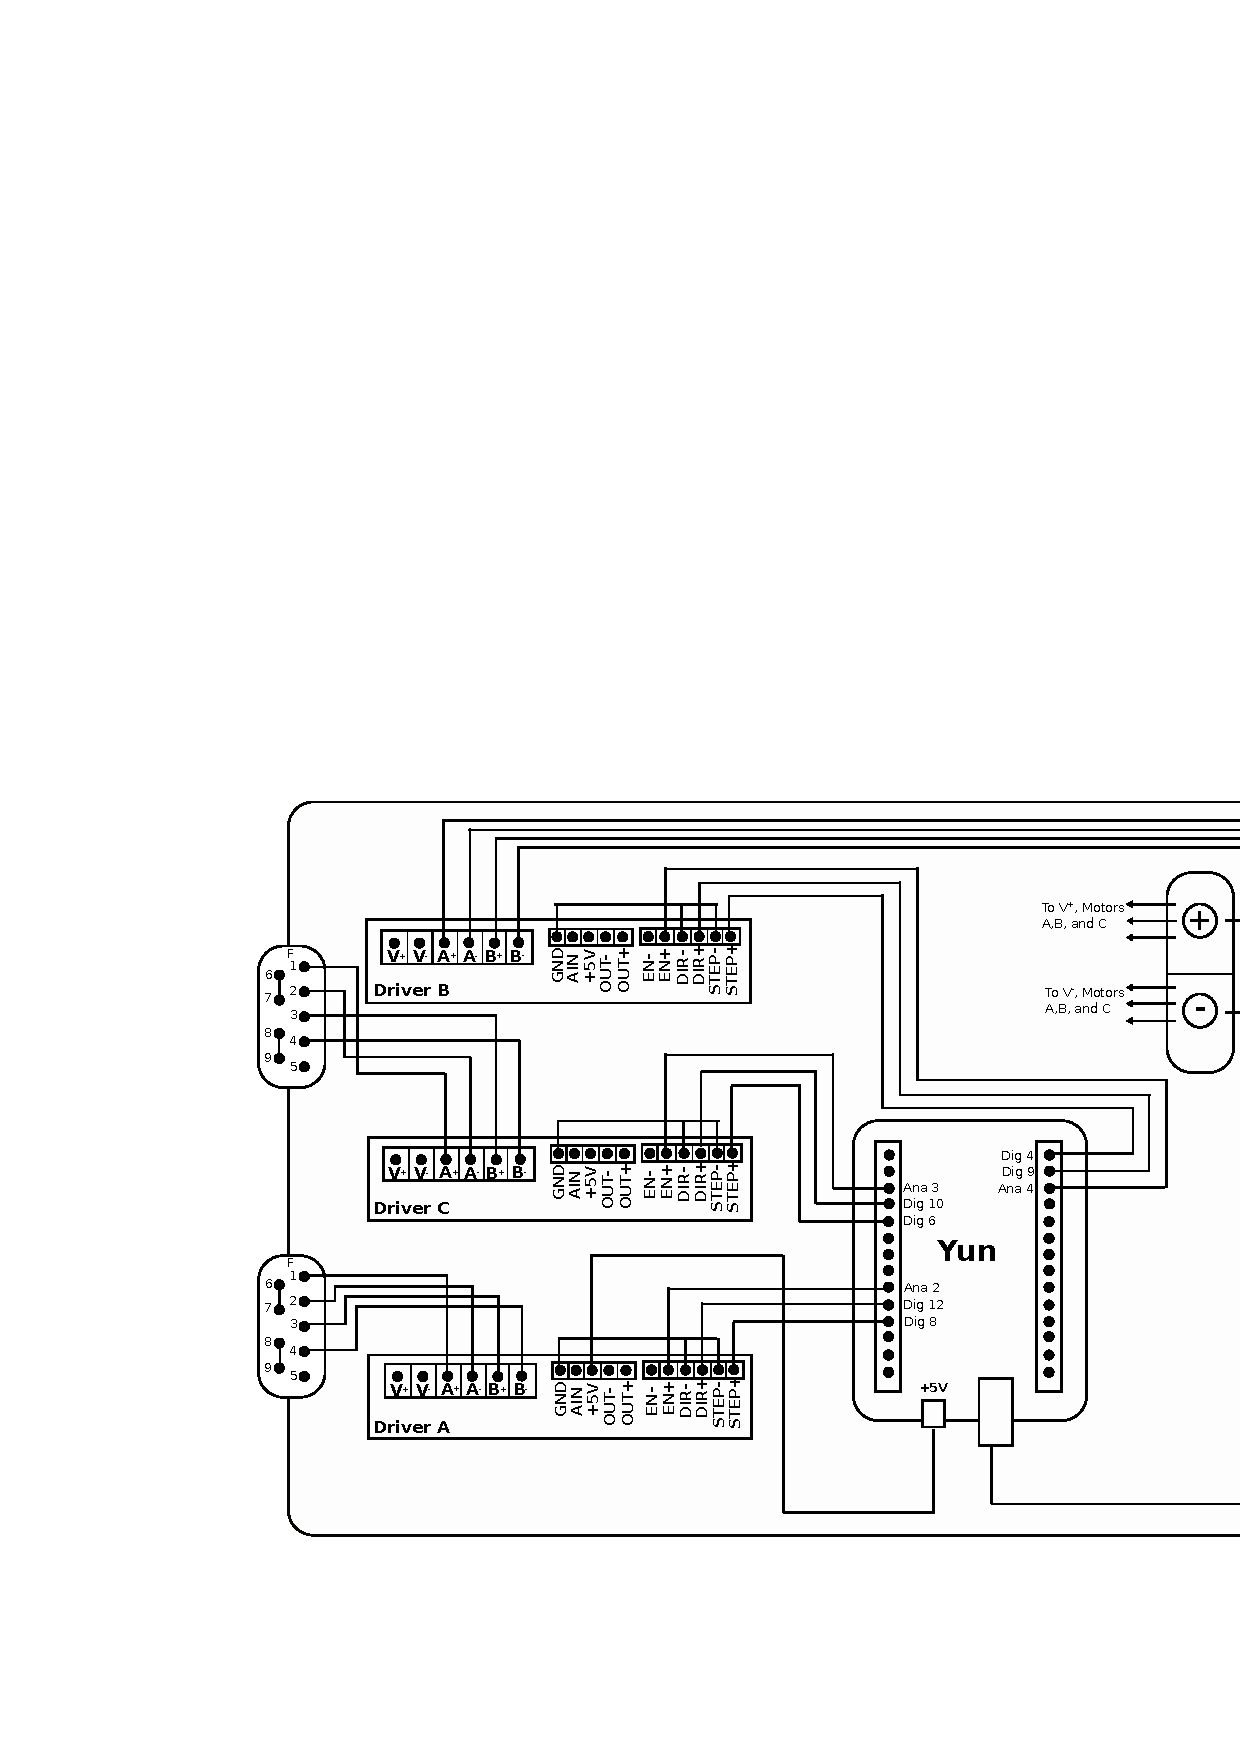
\includegraphics[width = 5in]{wiringDrawing.pdf}
\end{center}
\caption{Wiring Diagram}  
\label{fd2}
\end{figure}

\end{document}
